 \documentclass{revtex4}
% All LaTeX commands are preceded with a backslash, and every LaTeX document
% must begin with ``\documentclass'' declaration, which specifies which desired
% style file LaTeX should use.  Here we are using the style file (revtext4)
% adopted by the American Physics Society (APS).  See
% http://journals.aps.org/revtex for details.

% Note that comments begin with a "%" and are not turned into text in the .pdf
% document.  Comment blocks can be arbitrarily long.

% Next, we (optionally) declare which external packages we would like to use. The graphics package here allows us to import jpg and png figures into our document.
\usepackage{graphicx}

% The \begin{document} and \end{document} commands (obviously!) tell LaTeX where
% the document begins and ends, so these commands are mandatory.
\begin{document}

% Your document should have a descriptive title.
\title{Example Lab Report: Choose a Descriptive Title}

% The ``~`` in between my first initial and last name is an empty space but it forces LaTeX to not split the line between ``J.'' and ``Moustakas''.  Handy trick!
\author{John~Moustakas} 
\author{Albert~Einstein}
\author{Richard~Feynman}
\affiliation{PHYS 310}

\date{2016 Sep 3} % You can use \today{} or simply enter the date.

\begin{abstract}
The list of authors should include your name first and your group members ("coauthors") next, in alphabetical order. The abstract should contain a brief, one-paragraph summary which motivates the goals of the experiment or project (the "why"), summarizes your procedure (the "how"), and describes your results (the "what") and conclusions (the "so what").
\end{abstract}

% This line will actually create the title, author list, affiliation, and date.
% This command needs to occur *after* the abstract.
\maketitle

% Divide your write-up into logical sections (or even subsections, using
% the \subsection{My Subsection} command.
\section{Introduction}

The introduction should describe and motivate the purpose of the experiment or research project. Think of this section as an inverted pyramid: start with the big picture in order to provide the reader with context, and then focus down to the specific experiment or research question, and its objectives. The introduction should also answer the question of \emph{why} the experiment was necessary: what did we \emph{not} know before you carried out the project that required your time and effort?

Some additional tips:
% LaTeX tip: You can also make a numerical list using the "enumerate" environment.
\begin{itemize}
\item{Don't start too broad; focus on providing relevant information which is essential for understanding your project and results.}
\item{Cite any relevant previous literature on the subject in this section. This point is more for research papers rather than lab reports; don't worry about citing Galileo and Newton!}
\item{Consider writing this section last, after you have all the other pieces in place.}
\end{itemize}

\subsection{Adding a Subsection}

If your introduction (or any other section) is especially long then you can (optionally) add a subsection.

\section{Procedure}

This section should tell a story of what you did and what you found, including your experimental setup and all the equipment you used.  You should write this in narrative form, not as a list.  You may include a figure or two if appropriate (see \S~\ref{sec:analysis} for how to include a figure in your document), and there should be enough detail for another scientist (or student) to reproduce your experiment or experiments.

\section{Data}

% Note the \ref{} and \label{} macros allow you to refer to tables, figures, sections, etc. in the correct order even if you move them around.
This section should tabulate your measurements (data) or observations. Creating a table (see Table~\ref{tab:data}) is pretty straightforward.  You just need to specify how many columns you want and then put in the data! Note: (1) tables should have a clear and descriptive title; (2) columns should be labeled with the units noted at the top of each column; and (3) each table should be referenced in the text.

\begin{table}[h]
\centering
\begin{tabular}{lcc}
\hline
  & Mass $M$ & Radius $R$ \\
Planet & ($\times10^{24}$~kg) & (km) \\
\hline
\hline
Mercury & 0.3302 & 2439.7 \\
Venus   & 4.8676 & 6051.8 \\
Earth   & 5.9726 & 6378.1 \\
Mars    & 0.6417 & 3389.5 \\
\hline
\end{tabular}
\caption{Data on the four terrestrial planets. \label{tab:data}} 
\end{table}

% Note how I'm labeling this section so I can allude to it above.
\section{Analysis}\label{sec:analysis}

This section should contain a description of your analysis and results, including visualizations (figures) of your data and any derived quantities. You should also state any simplifying assumptions that you had to make.  

Every figure should have:
\begin{itemize}
\item{Well-labeled axes (including a large enough font to be readable);}
\item{Uncertainties on each data point;}
\item{A legend (if necessary);}
\item{And a succinct caption.}
\end{itemize}

In addition, every figure should be referenced in the main text and the main point or points you're trying to convey with the figure should be summarized.  In other words, be sure to describe not only the "what" but also the "so what" of the figure. 

To include a figure we use the {\tt figure} environment. For example, you might say that Figure~\ref{fig:example} shows my data and best-fitting line; it is a very nice
red line.
\begin{figure}[!h] % The ``!h'' means to insert the figure ``right here!''
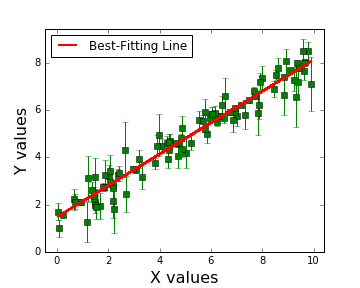
\includegraphics[height=3in]{example-figure.png}
\caption{Measurements of $Y$ as a function of $X$ (green points with error bars) with the best-fitting linear model (red line) overlaid. \label{fig:example}}
\end{figure}

Sometimes in this section you will need to show one or more derivations. These can be achieved using equations in the {\tt equation} or {\tt eqnarray} environments. For example, here's a one-line equation:
\begin{equation}
y = 4x + 7x^{2}
\end{equation}

\noindent And here's a multiline example:
\begin{eqnarray}
y & = & 4x + 3x + 6x \\
  & = & 7x + 6x \\
  & = & 13x
\end{eqnarray}

\noindent Alternatively, you can include an equation inside the text thusly: $e^{i\pi} + 1 = 0$.

\section{Discussion}

In this section you should assess the statistical significance of your results and interpret them in the context of previous work, current models or theories. Do not introduce any new data! In general this is the hardest section to write because you should draw on not only your own results, but also previous findings or ideas (citing relevant papers or texts as necessary). Citing a paper from the literature, like \citet{feynman69a} is easy!  Finally, you should almost always write this section after writing the Results section.

\section{Conclusions}

The conclusion should reinforce the major claims or interpretation in a way that is not mere summary. The writer should try to indicate the significance of the major claim/interpretation beyond the scope of the paper but within the parameters of the field. The writer might also present complications the study illustrates or suggest further research the study indicates is necessary.

% Import the bibliography.
\bibliography{bibliography}

\end{document}


